% =============================================================================
% File:  intro_git.tex -- Introduction to Git 
%
% =============================================================================

\documentclass[10pt,xcolor=dvipsnames]{beamer}

\usetheme{Madrid}

%\renewcommand\mathfamilydefault{\rmdefault}
\usefonttheme[onlymath]{serif}

%\usecolortheme{seahorse}
\usepackage[utf8]{inputenc}
\usepackage{xcolor}
\usepackage{colortbl}
\usepackage{verbatim}
\usepackage{hyperref}
%gets rid of bottom navigation bars
\setbeamertemplate{footline}{}
%gets rid of navigation symbols
\setbeamertemplate{navigation symbols}{}
%\usetheme{Frankfurt}
%\usetheme{Rochester}
%\usepackage{beamerthemeshadow}

% \usepackage{amsmath}
% \usepackage{amssymb}

%\usepackage{floatflt}
%\usepackage[utf8]{inputenc}
%\usepackage{multirow}
    \usepackage{mathptmx}
\graphicspath{{./pics/}{./figs/}}
\usepackage{graphicx}          % Include this line if your 
                               % document contains figures,
\usepackage[super]{nth}
\usepackage{multirow}
\usepackage{amsmath}
\usepackage{verbatim}


\AtBeginSection[]
{
  \frame{
    \frametitle{Summary}
    {\scriptsize\tableofcontents[currentsection]}
  }
}


%%%%%%%%%% Header %%%%%%%%%%%%
\title{Short Introduction to Git}
\subtitle{Group Seminar}

\author{Andr\'as Hartmann, Sascha Zickenrott}
\institute[LCSB]{
LCSB, Computational Biology group
  University of Luxembourg
}
% Mandatory to **declare** a logo to be placed on the bottom right -- normally the
% university logo. ADAPT ACCORDINGLY:

\date[June 29, 2016]{June 29, 2016, Luxembourg}

\logo{
\includegraphics[height=0.10\paperheight]{logo_UL.pdf} \hspace{0.2in}\vspace{0.2in}}

%%%%%%%%%%%%% Body %%%%%%%%%%%%%%%
\begin{document}

\begin{frame}
  \vspace{2.5em}
\begin{center}
    
\includegraphics[height=0.2\textheight]{git-logo.jpg}
\end{center}
  \titlepage
\end{frame}

\frame{
	\frametitle{Content}
	{\scriptsize\tableofcontents}
}

\section{Introduction}

\begin{frame}{Why use Version Control Systems?}
\begin{itemize}
\item Version Control = Revision Control = Source Control
\item Allows you to track your files over time on a standardized (foolproof) way.
\item Ever get files like Final\_rev.22.comments49 ... doc?
\end{itemize}
\centering
    
\includegraphics[height=0.6\textheight]{Finaldoc.png}
\end{frame}

\begin{frame}{Why use Version Control Systems?}
    \begin{columns}
        \column{0.5\textwidth}
\begin{itemize}
\item Collaboration
	\begin{itemize}
	\item Sharing files
	\item Collaborative editing
	\item Review changes, trace problems
	\item Optimal team work-flow
	\end{itemize}
\end{itemize}
        \column{0.5\textwidth}
\begin{itemize}
\item Backup \& History
	\begin{itemize}
	\item Ultimate ctrl-z (undo)
	\item Remote / local storage
	\item Logs: comments to all revisions
	\item No more loosing your files
	\end{itemize}
\end{itemize}
    \end{columns}
\centering
    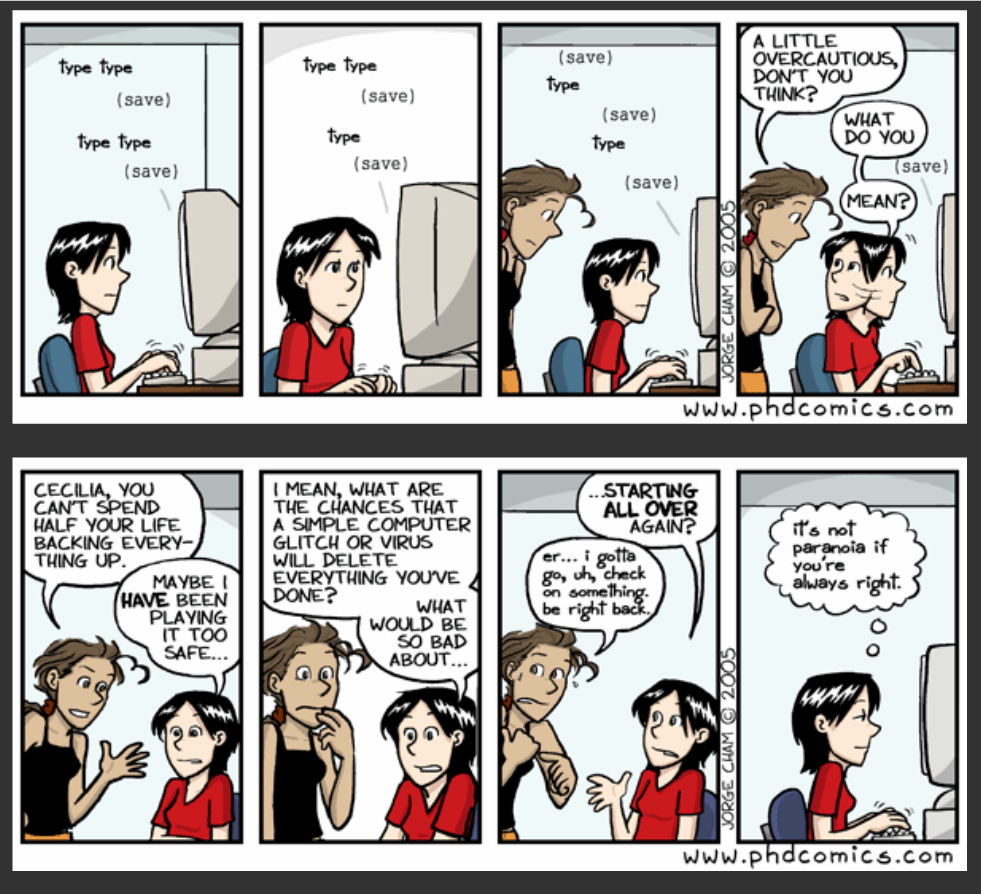
\includegraphics[height=0.6\textheight]{ctrl-s.png}
\end{frame}

\begin{frame}{What kind of data?}{Version Control Systems}
\begin{itemize}
  \setlength\itemsep{0.4in}
\item Mainly {\bf text} files\\
- Source code, txt files, \LaTeX\  source, etc ...
\item No sophisticated difference for binary files\\
- Word, Excel documents, pictures, pdfs ...
\item For \LaTeX\ collaborative editing you may want to try\\
- sharelatex: https://www.sharelatex.com
\end{itemize}
\end{frame}



\begin{frame}{Why git?}
\begin{itemize}
\item Decentralized / Distributed
\item Fast
\item Flexible
\item Works offline
\end{itemize}
~\\[0.2in]
\centering

\includegraphics[width = 0.8\textwidth]{companies.png}\\
\end{frame}
\section{Git basics}

\begin{frame}{Local vs Centralized VCS}
\begin{columns}%TODO align columns
\column{.5\textwidth}
\centering
{\LARGE LOCAL}\\[0.2in]
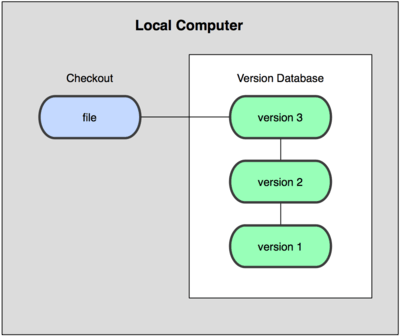
\includegraphics[scale=0.3]{VCS_local.png}\\
Not shared with anyone\\
e.g. on your own HDD
\column{.5\textwidth}
\centering
{\LARGE CENTRALIZED}\\[0.2in]
%{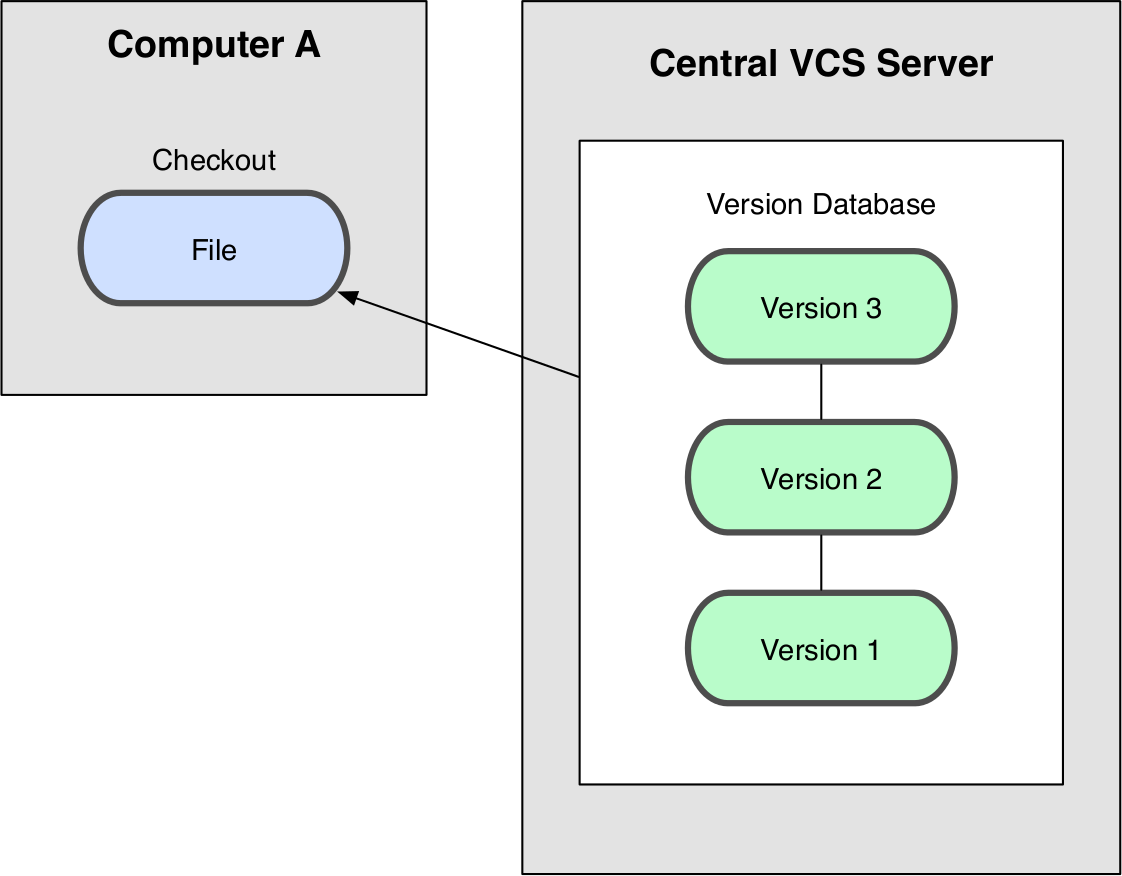
\includegraphics [scale=0.3]{VCS_centralized-1.png}}
{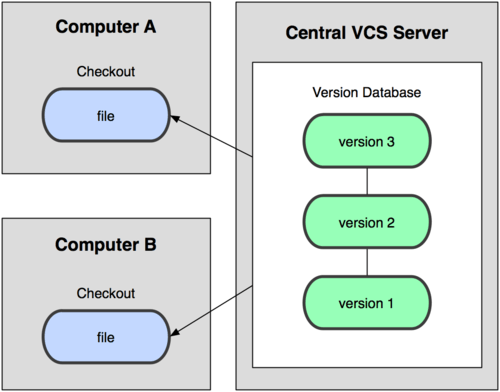
\includegraphics [scale=0.3]{VCS_centralized-2.png}}\\
Everybody sees the same version\\
on the server\\
\end{columns}
\end{frame}

\begin{frame}{Distributed VCS}{Git}

\begin{center}
\centering
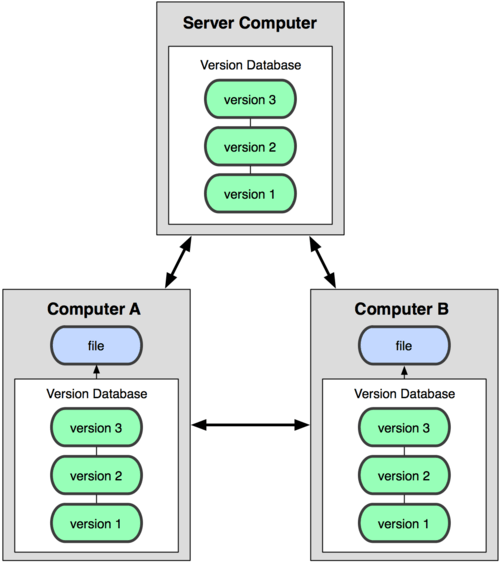
\includegraphics [scale=0.3]{VCS_distributed.png}\\[0.2in]
Both local AND global, but most operations are local\\
 Everybody has the full history of commits
\end{center}
\end{frame}

\begin{frame}{Tracking changes}
\centering
{\LARGE Most VCS}\\[0.1in]
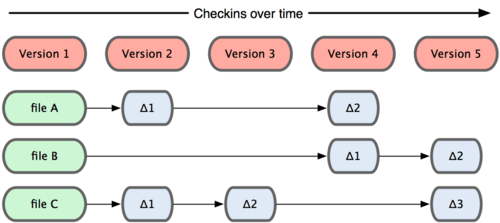
\includegraphics [scale=0.3]{tracking_changes_svn.png}\\[0.2in]
\pause
{\LARGE Git}\\[0.1in]
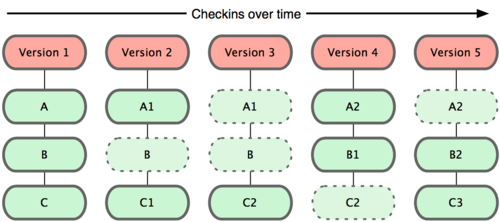
\includegraphics [scale=0.3]{tracking_changes_git.png}\\[0.1in]
``Git thinks of its data more like a set of snapshots of a mini filesystem.''
\end{frame}



\subsection{Install}

\begin{frame}{Install git}
\begin{block}{Linux / UNIX}
     \begin{itemize}
       \setlength\itemsep{0.2in}
       \item {\bf OS X}\\ \$ brew install git %#\;\;\;\;\; #homebrew
       \item {\bf Ubuntu}\\ \$ aptitude install git
       \item {\bf Arch}\\ \$ pacman -S git
     \end{itemize}
\end{block}

\begin{block}{Windows}
    \begin{itemize}
      \item \url{https://git-for-windows.github.io/}
    \end{itemize}
\end{block}
\end{frame}

\subsection{Commands}

\begin{frame}{The three (local) Stages}
\begin{center}
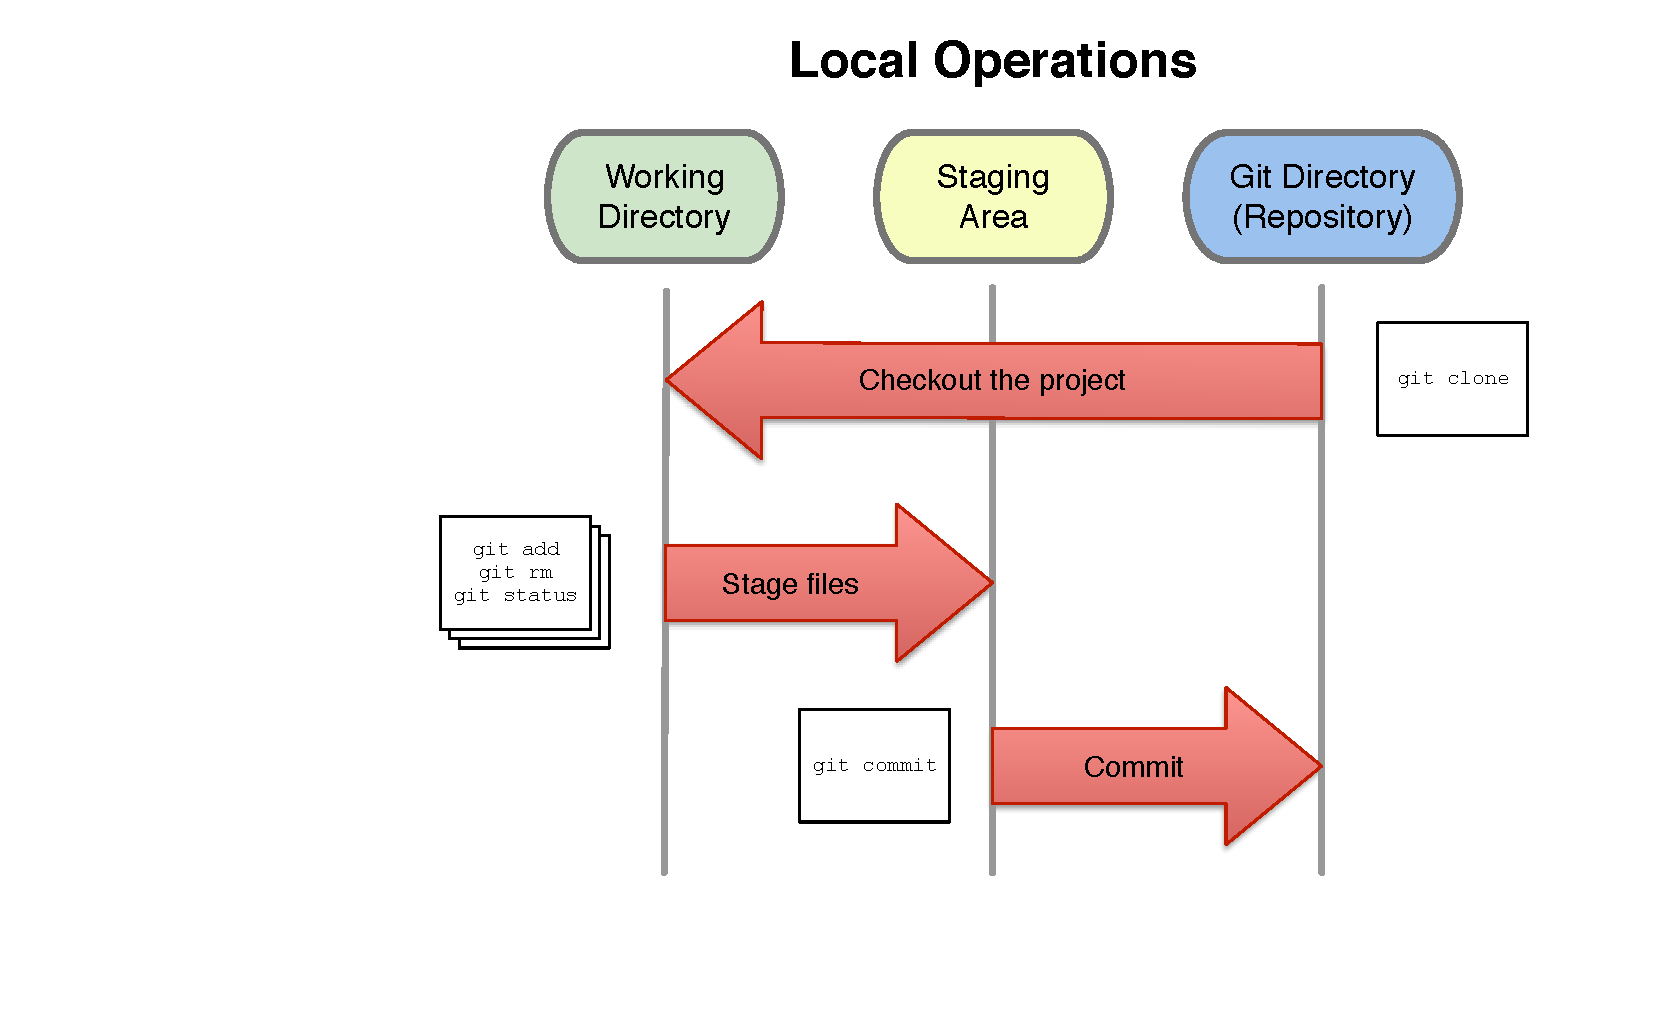
\includegraphics[width = 0.7\textwidth]{three_states.pdf}
\end{center}
\begin{itemize}
\item The {\bf local repository} lives in the .git directory.
\item The {\bf staging area} tracks what will go into the next commit, kind of index
\end{itemize}
\end{frame}



\begin{frame}{First steps}
\begin{block}{}
\$ git init
\end{block}
Initializes a new git repository\\[0.4in]

\begin{block}{}
\$ git clone [–-recursive] $<$url$>$ [$<$path$>$]
\end{block}
Clones a remote repository to access locally\\
url can be local /git / git+ssh / http(s), etc ...
\end{frame}

\begin{frame}{Adding new files}
\begin{block}{}
\$ git add [-f] [$<$pathspec$>$ ...]
\end{block}
Adds new file(s) to the index
\begin{center}
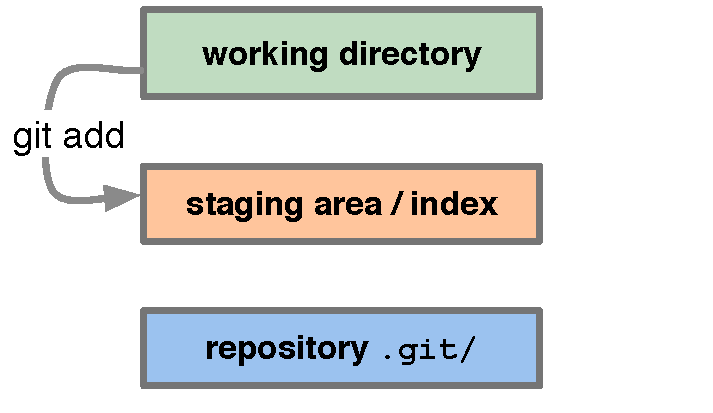
\includegraphics[scale=0.3]{diagrams_add_commit-02.pdf}
\end{center}
\end{frame}

\begin{frame}{Committing changes}
\begin{block}{}
\$ git commit [-a] [-m "msg"] [$<$pathspec$>$ ...]
\end{block}
Commits the changes\\
-a: commits all,
-m: write a message
\begin{center}
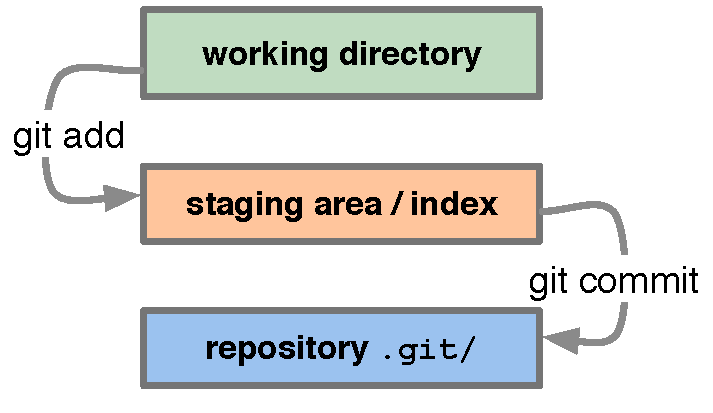
\includegraphics[scale=0.3]{diagrams_add_commit-03.pdf}
\end{center}
\pause
{\bf IMPORTANT}:
\begin{itemize}
\item Always write a descriptive message to your commit!
\item In the commit description list all files you changed, and describe why
\item In general, try to commit often, commits are save points
\item Do not commit code that does not run
\end{itemize}

\end{frame}

\begin{frame}{Moving / deleting files}
\begin{block}{}
\$ git rm [-rf] [-- cached] [$<$pathspec$>$ ...]
\end{block}
--cached : removes from Staging area\\
default: from index {\bf and} file system\\[0.4in]
\begin{block}{}
\$ git mv $<$source$>$ $<$destination$>$
\end{block}
Moves source to destination
\end{frame}

\begin{frame}{Status / diff }
\begin{block}{}
\$ git status 
\end{block}
Show the working tree status: differences between the index file and current HEAD commit\\[0.4in]
\begin{block}{}
\$ git diff [--cached] [$<$ref$>$][$<$pathspec$>$ ...]
\end{block}
Check un-staged changes (line by line)\\
-- cached: check staged changes\\
Can be relative to a revision, like 1776b2, or HEAD\\[0.4in]

In general it is a good practice to check status and diff {\bf before} commiting
\end{frame}

\begin{frame}{log / blame }
\begin{block}{}
\$ git log [--since="date"] [$<$pathspec$>$ ...]
\end{block}
time-filtering: --since=2.weeks or\\
--since="2 years 1 day 3 minutes ago"\\[0.4in]

\begin{block}{}
\$ git blame $<$file$>$ 
\end{block}
Who was it?
\end{frame}


\begin{frame}{Undo / ctrl-z}
\begin{block}{}
\$ git commit –-amend
\end{block}
Changes the last commit
\begin{block}{}
\$ git unstage $<$file$>$ \\
\$ git reset HEAD $<$file$>$
\end{block}
Unstage staged file
\begin{block}{}
\$ git checkout $<$file$>$
\end{block}
Restores file to last commit. DANGER: all the changes lost!
\begin{block}{}
\$ git revert $<$commit$>$
\end{block}
Reverts a $<$commit$>$: makes a new commit that undoes \\ {\bf all} the changes made in $<$commit$>$
\end{frame}

\begin{frame}{.gitignore}
If present in a folder, tells git to ignore files
\begin{block}{.gitignore example}
*.pyc\\
%*\~\\
*.swp\\
/build/\\
/doc/[abc]*.txt\\
.pypirc\\
*.egg-info\\
\end{block}
\begin{itemize}
\item Blank lines or lines starting with \# are ignored (comments)
\item Standard glob patterns work (wildcards)
\item End pattern with slash (/) to specify a directory
\item Negate pattern with exclamation point (!) 
\end{itemize}
\end{frame}
\subsection{Working with remote(s)}

\begin{frame}{Remotes}
\begin{center}
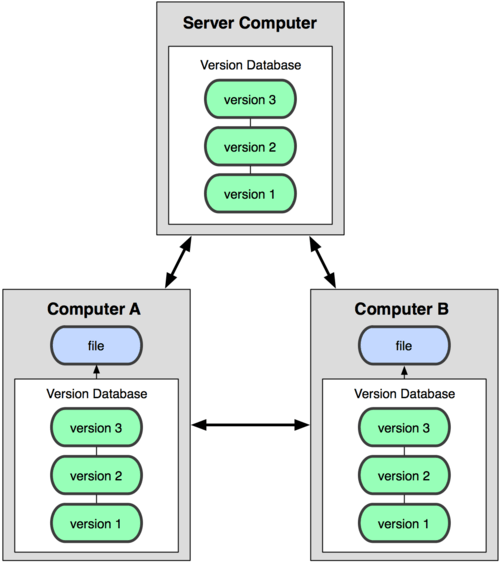
\includegraphics [scale=0.2]{VCS_distributed.png}\\[0.2in]
\end{center}
\begin{itemize}
\item Other clones of the same repository
\item Can be local (another checkout) or remote (coworker, central server)
\item There are default remotes for push and pull 
\end{itemize}
\begin{block}{}
\$ git remote -v \\
origin git://github.com/schacon/ticgit.git (fetch) \\
origin git://github.com/schacon/ticgit.git (push)
\end{block}
\end{frame}

\begin{frame}{Remotes}

\begin{block}{}
\$ git pull $<$remote$>$ $<$rbranch$>$
\end{block}
Or simply:\\
\$ git pull\\
Pulls the commits from the remote\\[0.2in]

\begin{block}{}
\$ git push -u $<$remote$>$ $<$rbranch$>$
\end{block}
Using defaults:\\
\$ git push -u origin master\\
Pushes all the commits into the remote\\[0.2in]
{\bf IMPORTANT}: do not simply push to someone else's repository\\
create a pull request instead
\end{frame}


\begin{frame}{Local vs Remote}
\begin{center}
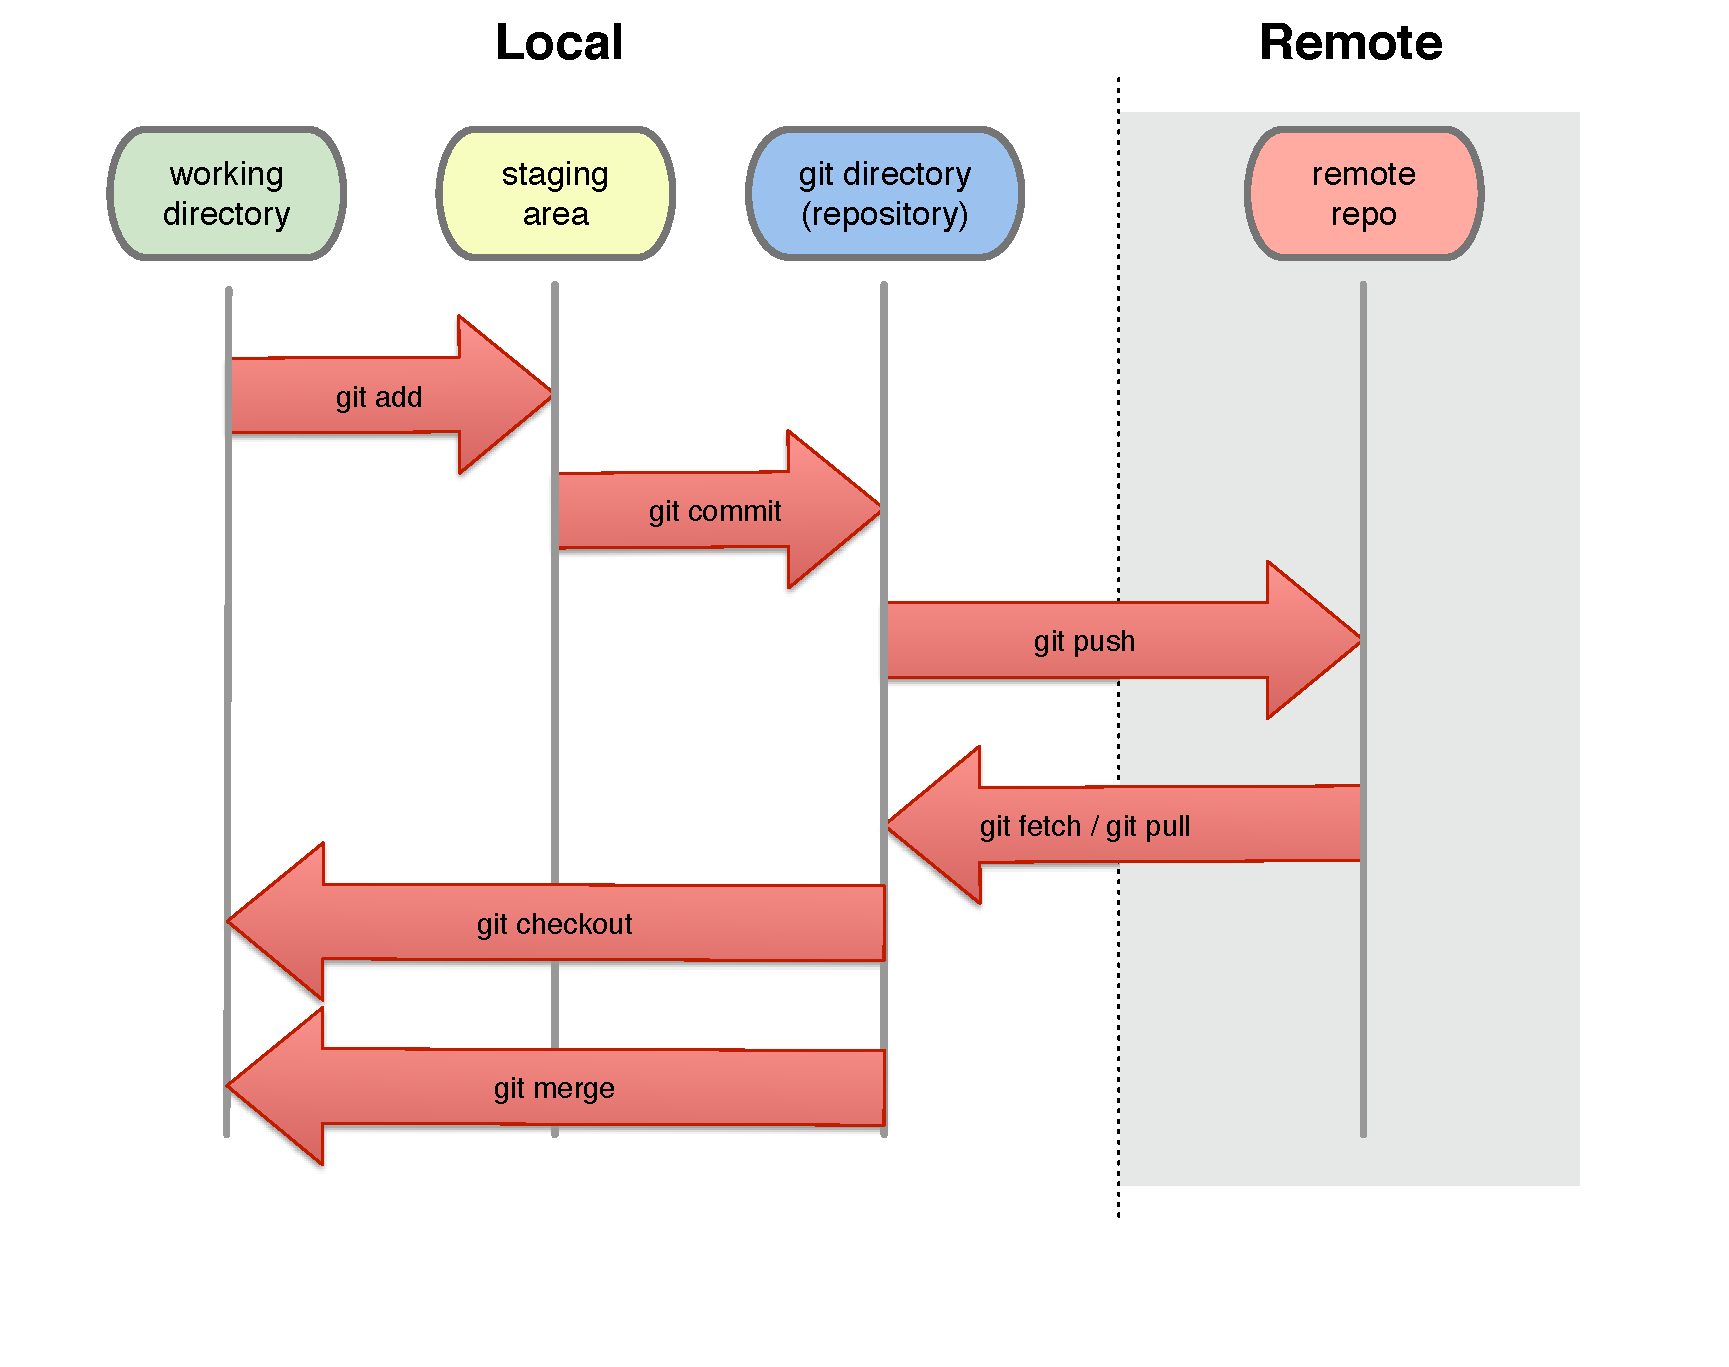
\includegraphics[width = 0.7\textwidth]{diagrams-lifecycle_remote.pdf}
\end{center}
\end{frame}

\subsection{Branches}

\begin{frame}{Branches}
\begin{itemize}
\item Branches are ``Pointers'' to commits
\item Branches can diverge during development
\end{itemize}
~\\[0.1in]
\begin{center}
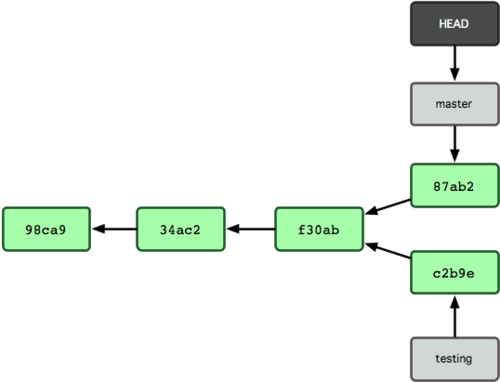
\includegraphics[width = 0.6\textwidth]{branch2.png}
\end{center}
\end{frame}

\begin{frame}{Branches}
\begin{center}
\begin{itemize}
\item Merge: ``joining branches'': usually painless
\item Conflicts the same line has changed 
\begin{itemize}
\item Have to be resolved (manually / automatically)
\end{itemize}
\end{itemize}
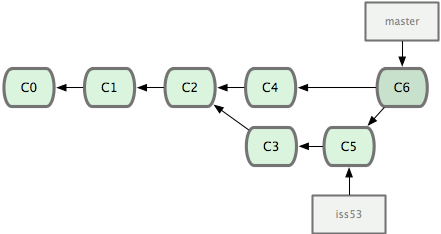
\includegraphics[width = 0.6\textwidth]{branchmerge.png}
\end{center}
\end{frame}

\begin{frame}{Some Typical VCS Workflows}
\begin{columns}
\column{.5\textwidth}
{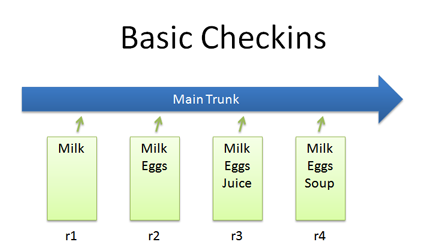
\includegraphics [scale=0.3]{basic_checkin.png}}
\pause
{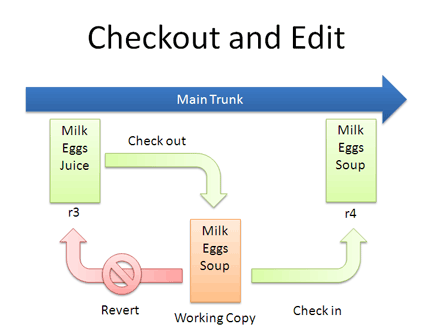
\includegraphics [scale=0.3]{checkout_edit.png}}
\pause
\column{.5\textwidth}
{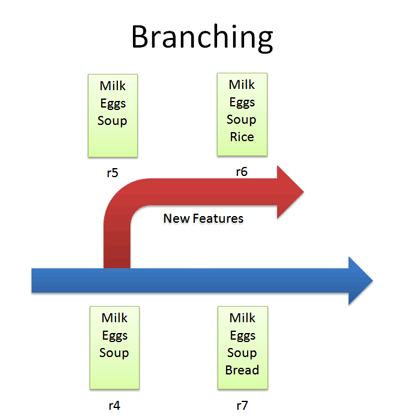
\includegraphics [scale=0.28]{first_branch.png}}
\pause
{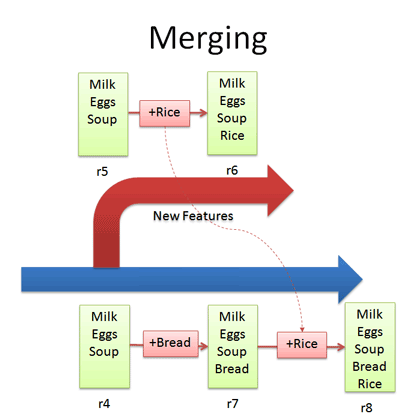
\includegraphics [scale=0.28]{merging.png}}
\end{columns}
\end{frame}

\section{GitLab}
\begin{frame}{GitLab}
\begin{itemize}
\item GitLab is an online git interface (like github)\\
\item Available at \url{https://git-r3lab.uni.lu}\\[0.2in]
\end{itemize}
\centering

\includegraphics[height=0.70\paperheight]{gitlab.png} 
\end{frame}

\section{Git resources}
\begin{frame}{Further reading}
\begin{itemize}
  \setlength\itemsep{0.2in}
\item "Pro Git" Book by ... \\$\rightarrow$  \url{http://git-scm.com/book}
\item Git reference  \\ $\rightarrow$  \url{http://git-scm.com/docs}
\item Git cheatsheet  \\ $\rightarrow$ \url{https://www.git-tower.com/blog/git-cheat-sheet}
\item This presentation is on github\\
\$ git clone \url{https://github.com/AndrasHartmann/gitprez.git}
\item You can always check:\\
 \$ help git [$<$command$>$]
\end{itemize}
\end{frame}

\begin{frame}{Learning by doing}
\begin{itemize}
  \setlength\itemsep{0.2in}
\item Tutorials  \\$\rightarrow$  \url{https://www.atlassian.com/git/tutorials}
\item Learn Git on codecademy - Strongly recommended!\\ $\rightarrow$ \url{https://www.codecademy.com/learn/learn-git}
\item Most important:
\begin{center}

\includegraphics[height=0.3\textheight]{fire-git.png}
\end{center}
\end{itemize}
\end{frame}

\end{document}
